\documentclass[dwyatte_dissertation.tex]{subfiles} 
\begin{document}

\sloppy

\chapter{Neural model of spatiotemporal prediction for object recognition}

\section{Introduction}
The work presented in this chapter describes a neural network model of the broader LeabraTI framework (Chapter \ref{chap:leabrati}). The specific implementation was used to investigate the role of spatiotemporal predictive learning in an object recognition task, analogous to the ones used in the Chapter \ref{chap:pleast} and \ref{chap:bpleast} experiments. The principal behavioral results of these experiments are first reviewed before turning to the model implementation and simulations that reproduce these results.

The Chapter \ref{chap:pleast} experiment investigated the role of predictive processing during a novel object recognition task. The experiment made use of novel three-dimensional ``paper clip'' objects that required integration over multiple sequential views to extract their three-dimensional structure. The results of the experiment indicated that spatial and temporal predictability of an entraining sequence enhanced discriminability of a subsequently presented probe stimulus using a same-different judgement.

The Chapter \ref{chap:bpleast} experiment expanded on the previous chapter's experiment by investigating the role that spatial and temporal predictability played during prolonged learning about the same paper clip objects. The experiment involved an explicit training period during which observers studied the objects while they were rotated through their views followed by a series of test trials that required same-different judgements about static probe stimuli. Somewhat surprisingly, the results of the experiment were an almost complete reversal of the previous chapter's experiment. Accuracy was lowest when stimuli were learned in a combined spatially and temporally predictable context and highest when learned in a completely unpredictable context.

The model described next was capable of producing the results of both experiments. LeabraTI makes the fundamental prediction that spatially predictable sequences presented at a regular temporal interval offset with the brain's endogenous 10 Hz predictions should maximally activate representations due to the multiple successful prediction-sensation events. The result is a superadditive effect for spatiotemporally predictable sequences, which has also been demonstrated in previous investigations of predictability on attentional allocation \cite{DohertyRaoMesulamEtAl05,RohenkohlGouldPessoaEtAl14}. The reversal effect due to prolonged learning was able to be produced by increasing the scale of a single projection of synaptic weights in the model. 

\section{Methods}

\subsection{Model architecture}

The model architecture is illustrated in Figure \ref{fig:v1_v2_output}. The model consisted of three layers and one preprocessing stage whose parameters are described in detail in the following paragraphs. Two of the layers contained columnar substructure necessary for learning using the LeabraTI algorithm. To simplify the overall LeabraTI computation, only superficial (Layers 2 and 3) and deep (Layer 6) neuron subtypes were explicitly modeled. Projections between these neuron populations corresponded to the descending Layer 5 $\rightarrow$ Layer 6 synapses in the brain, which are assumed to be plastic, and the ascending Layer 6 $\rightarrow$ Layer 4 transthalamic synapses which are assumed to be relatively stable and nonplastic. This simplification captures the core computational properties of the LeabraTI framework while reducing the overhead of simulating the full columnar substructure of the neocortex.

% model fig
\begin{figure}[h!]
\begin{center}
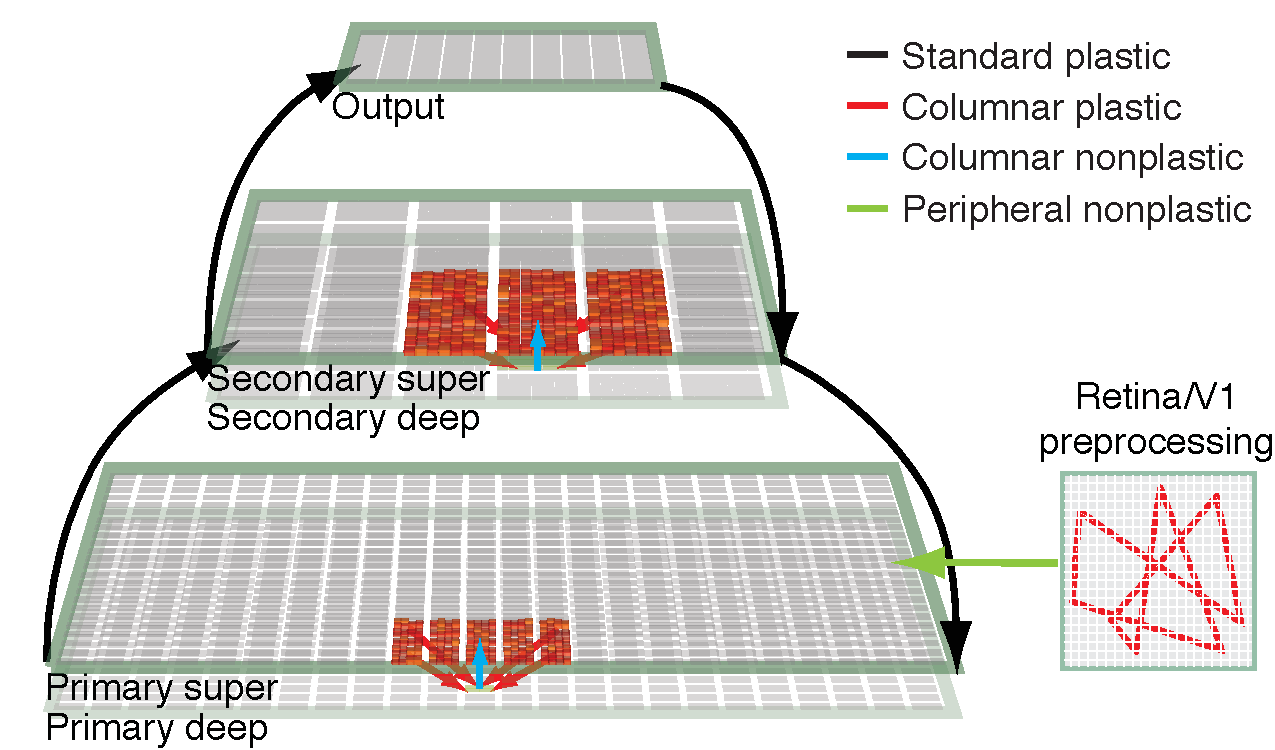
\includegraphics[width=160mm]{figs/chap_sims/v1_v2_output_ti_annotated.pdf}
\end{center}
\caption{Model architecture}{The model's four layers and principal projections. Primary and secondary visual layers contained columnar substructure in which deep units integrated from 5x5 columns of superficial units in the primary case or 3x3 columns in the secondary case. Ascending synapses from deep to superficial units were nonplastic and connected in a one-to-one manner.}
\label{fig:v1_v2_output}
\end{figure}

% retina/v1 prep roc actually uses new FFFB inhibition -- check new LaebraAppendix.tex for description, revise here
\textbf{Retina and V1 preprocessing:} Input was provided to the model via a 24x24 topographic filter bank that preprocessed images offline from the model proper. This preprocessing step is consistent with a large class of biological models describing object recognition in cortex \cite[e.g.,]{RiesenhuberPoggio99,SerreOlivaPoggio07,OReillyWyatteHerdEtAl13} and in the case of the present model, represents visual processing from the level of the retina through V1 simple cells \cite{HubelWiesel62}. Grayscale bitmap images were scaled to 24x24 pixels and convolved with Gabor filters at four orientations (0$^\circ$, 45$^\circ$, 90$^\circ$, and 135$^\circ$) and two polarities (off-on and on-off) producing a 24x24x4x2 set of inputs. Each Gabor filter was implemented as 6x6 pixel kernel, with a wavelength $\lambda$ = 6 and Gaussian width terms of $\sigma_x$ = 1.8 and $\sigma_y$ = 1.2. A static nonlinearity was applied to the output of the filtering step in the form of a modified \textit{k}-Winners-Take-All (\textit{k}WTA) inhibitory competition function that reduced activation across the 4x2 filter bank to the equivalent of \textit{k} = 1 fully active units \cite[see][Supporting Information]{OReillyWyatteHerdEtAl13}.

\textbf{Primary visual layers:} 24x24 topographic layer arranged into groups of 4x2 units (4608 total units), decomposed into superficial and deep neuron subtypes. Each superficial unit received the output of the retina/V1 preprocessing step. \textit{k}WTA inhibition for superficial units was set to 60\% of the average of the top \textit{k} active units compared to the average of all other superficial units with each 4x2 unit group using a value of \textit{k} = 2. Deep units received from 5x5 columns of superficial units (200 inputs per deep unit) integrated into a single value that was used as the additional context input channel for each superficial unit.

\textbf{Secondary visual layers:} 6x6 topographic layer arranged into groups of 7x7 units (1764 total units), also decomposed into superficial and deep neuron subtypes. Each superficial unit received from 8x8 topographical neighborhoods of early visual columns (512 afferents per unit) and sent back reciprocal connections with the same topography. \textit{k}WTA for superficial units was set to 60\% of the average of the top \textit{k} active units compared to the average of all other superficial units with each and 15\% activity within each unit group. Deep units received from 3x3 columns of superficial units (441 inputs per deep unit) integrated into a single value that was used as the additional context input channel for each superficial unit.

\textbf{Output layer:} 10x10 layer (100 total units) without unit group or columnar substructure. Each unit received a full projection from secondary visual columns (1764 afferents per unit) and fully projected back to all columns. A scale of 10\% was used to limit the influence of the output units on secondary visual columns during the training period, preventing ``hallucinatory'' representations that can become disconnected from bottom-up inputs. A \textit{k}WTA value of \textit{k} = 1 was used to enforce a localist representation. The localist representation is a computational simplification that allowed an identity readout of lower-level features without population decoding similar to that provided by inferior temporal (IT) neurons \cite{HungKreimanPoggioEtAl05,LiCoxZoccolanEtAl09}. 

\subsection{LeabraTI learning algorithm}

LeabraTI was implemented as an extension of the standard Leabra algorithm which is described in detail in \incite{OReillyMunakata00} and \incite{OReillyMunakataFrankEtAl12}. Standard Leabra learning operates across two phases: a \textit{minus} phase that represents the system's expectation for a given input and a \textit{plus} phase, representing observation of the outcome. The difference between the minus and plus phases, along with additional self-organizing mechanisms, is used in computing the synaptic weight update function at the end of each plus phase. 

LeabraTI extends standard Leabra learning by interleaving its minus and plus phases over temporally contiguous input sequences. In standard Leabra, the minus phase depends on clamped inputs from the sensory periphery to drive the expectation while the plus phase uses clamped outputs from other neural systems to drive the outcome. In LeabraTI, the minus phase expectation is not driven by the sensory periphery, but instead by lagged context represented by deep (Layer 6) neurons. During the plus phase, driving potential shifts back to the sensory periphery. Deep neurons' context is also updated after each plus phase.

LeabraTI was only used to update the synaptic weights between superficial and deep neurons. Inter-areal feedforward and feedback projections bifurcate from the local column, directly synapsing disparate populations of superficial neurons and thus weight updates in these cases were handled by standard Leabra equations. In computing the weight update, the standard Leabra delta rule \cite{OReilly96} uses the difference in rate between the plus and minus phases of receiving units (\textit{y}) in proportion to the rate of sending units (\textit{x}) in the minus phase:
\begin{align*}
\Delta_{leabra} w_{ij} &= x^-(y^+ - y^-)
\end{align*}

In the LeabraTI framework, deep neurons are considered to be the receiving units as they are the terminus of the descending columnar synapses. However, deep units are proposed to only be active during the minus phase when they drive the prediction, and thus cannot be used to compute an error signal.  To address this issue, we invert the LeabraTI delta rule:
\begin{align*}
\Delta_{leabrati} w_{ij} &= super^-(deep^+ - deep^-) \\
			  &\approx deep^-(super^+ - super^-)
\end{align*}

Additionally, the temporally extended nature of the algorithm requires that the receiving units represent the current state (time \textit{t}) and sending units the previous moment's state (time \textit{t} - 1). While conceptualized as the previous equation, the actual implementation is as follows:
\begin{align*}
\Delta_{leabrati} w_{ij} &= super_{t-1}^+(super_{t}^+ - super_{t}^-)
\end{align*}

This formulation allows the driving potential of deep neurons to be computed just once using the previous plus phase state of superficial neurons (multiplied by the superficial $\rightarrow$ deep learned weights) and held constant as an input to superficial neurons during the minus phase. This is a gross simplification of the actual biological process of deep neurons, but is vastly more computationally efficient than explicit modeling by computing an additional rate for each deep neuron at each time step. This formulation is also equivalent to the simple recurrent network (SRN) \cite{Elman90,Servan-SchreiberCleeremansMcClelland91}, thus providing a potential biological substrate for its computational function. 

One limitation of LeabraTI's interleaving of minus and plus phases over time is that the initial minus phase in an input sequence does not have access to the previous moment's  context. Even if there was lagged context available, it would represent information from a prior, possibly unrelated input sequence. To address this, weight updates are disabled for the first minus-plus phase pair, and enabled thereafter. In the brain, this process might be facilitated by a neural mechanism that is sensitive to the repetition of inputs over time (e.g., acetylcholine) \cite{ThielHensonMorrisEtAl01,ThielHensonDolan02}.

\subsection{Training and testing environment}
LeabraTI requires training to establish establish the spatial associations over subsequent time steps. In human development, this is expected to be facilitated by coarse transformations of retinal inputs due to environmental or self motion. This initial learning stage develops generic features that capture how inputs change from moment-to-moment (100 ms timeframes in LeabraTI). The actual inputs are not critical except that they accurately reflect the average statistics of the environment. In training the model, a simplified  ``paper clip'' environment was assumed, using the four objects from the Chapter \ref{chap:bpleast} experiment.

% 50 cycles -, 20 +
During training, an input sequence depicted one of the four objects rotating coherently through all 30 view renderings (adjacent views spaced 12 degrees apart). During the minus phase, the model made a prediction about the upcoming view and during the plus phase, the view was processed by the retina/V1 filter banks and clamped as an input to the model. The output unit corresponding to each object was also clamped during the plus phase to bias views belonging to the same object toward similar lower-level feature representations. Training proceeded for 20 epochs of 10 randomly selected input sequences each. The learning rate on all plastic synapses started at 1.0 and was halved every 8 epochs.

Training efficacy was evaluated by computing the average cosine (normalized dot product) between the minus and plus phase for the primary and secondary visual layers:
\begin{align*}
cos \theta = \frac{1}{n}\sum_{k=1}^{n}\frac{layer_k^- \cdot{} layer_k^+}{||layer_k^-||||layer_k^+||}
\end{align*}

The cosine varies between 0 and 1 and expresses the degree of similarity of LeabraTI's prediction to the actual outcome in layers with columnar substructure (Figure \ref{fig:sims_train}). A value of zero indicates the minus phase prediction is completely orthogonal to the plus phase sensation and a value of 1 indicates complete overlap. The lower-bound on the cosine is not likely to be zero as it would require spurious activations in topographic regions that do not contain any features. A better approximation of the lower bound is the case when the system simply reproduces the plus phase from the previous moment's (\textit{t} - 1) state. This can be thought of as the amount of perceptual overlap between adjacent views of the stimuli, and thus any additional features that contribute to a higher cosine value indicate positive prediction.

% training fig
\begin{figure}[h!]
\begin{center}
\begin{tabular}{ll}
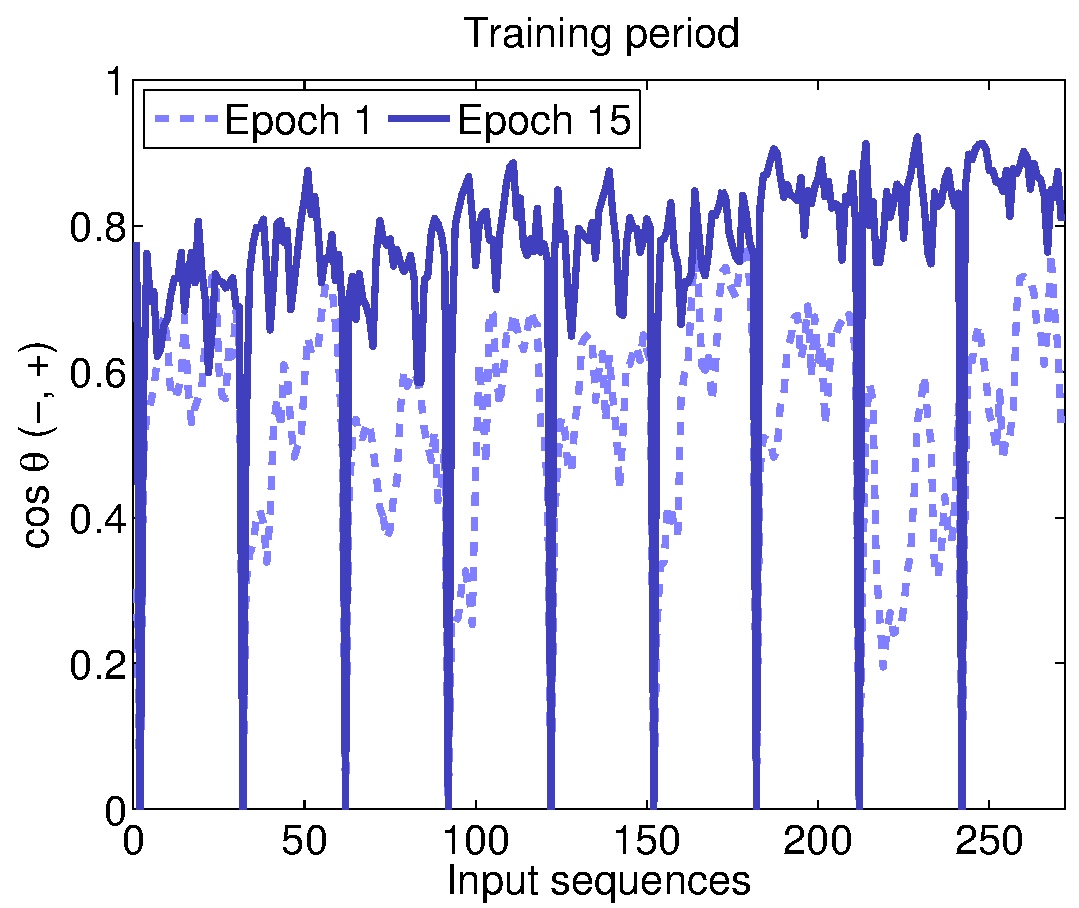
\includegraphics[width=80mm]{figs/chap_sims/sims_cos_out_trl.pdf}
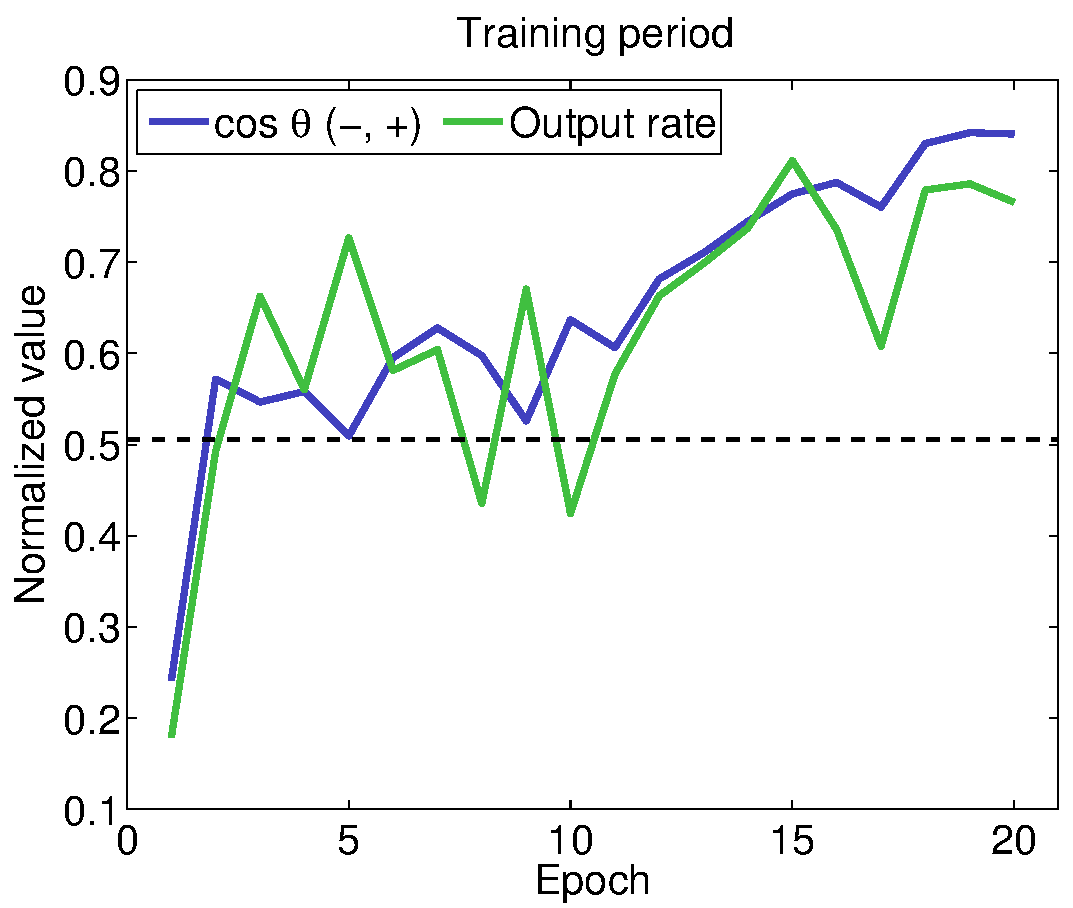
\includegraphics[width=80mm]{figs/chap_sims/sims_cos_out_epc.pdf}
\end{tabular}
\end{center}
\caption{Model training}{Average cosine between minus and plus phase for layers with columnar substructure and output response rate over the course of training. Sharp drops in the cosine to zero indicate the start of a new input sequence and are unlearnable. The lower bound for the cosine was computed as the reproduction of the plus phase from the previous moment's (\textit{t} - 1) state and the overall average is indicated by the dotted line. A cosine greater than this level indicates positive prediction.}
\label{fig:sims_train}
\end{figure}

Typically, after the initial feature training phase, neural models are trained to classify stimulus-response pairs (\nopcite{RiesenhuberPoggio99,SerreOlivaPoggio07}; although, see also \nopcite{OReillyWyatteHerdEtAl13}). In human learning, stimulus predictability and response mappings can be learned independently \cite{WyartNobreSummerfield12,KokRahnevJeheeEtAl12}. The present model was compact and input environment simple enough that the initial features and response mappings could be learned jointly. The rate of the target output unit was used to evaluate the efficacy of the learned response mappings. 

Consistency between features and responses was ensured by using two sets of synapses with different update intervals that contribute a weighted mixture to the input of each receiving unit. The first ``standard'' set of synapses were updated after every plus phase, whereas a second ``stable'' set of synapses were updated at the end of each epoch. In the present model, a 80\% stable to 20\% standard synaptic mixture was used. This allowed the model to more slowly integrate learning across an entire epoch's worth of input sequences without runaway representations caused by being exposed to the same rotating object's features over multiple time steps while still maintaing the moment-to-moment spatiotemporal predictive learning central to LeabraTI.

Testing involved presenting input sequences accordant with each of the four predictability conditions used in the Chapter \ref{chap:pleast} and \ref{chap:bpleast} experiments. In the spatially unpredictable conditions (S-), random views were selected for each plus phase and used to compute deep neurons' updated context. To model the effect of temporal unpredictability (T-), a variable number of time steps (up to four) separated each context update. Each time the context update was skipped, a decay factor of 50\% was applied to superficial neurons' context input channel. The default scale of this channel was 100\% and thus four time steps without a context update decayed the scale to 12.5\%. The net effect of temporal unpredictability was a weakening of the prediction at each time step until the next view was actually presented and the updated context could be computed.

The completely unpredictable condition (S-T-) utilized both the variable update interval and decay whereas the combined spatial and temporal predictability condition (S+T+) was identical to the training procedure (i.e., a coherently rotating object with constant update interval). In all cases, predictions about each upcoming view were made during each minus phase given the current context state. Weight updates that normally occurred at the end of each plus phase during training were disabled on all plastic synapses during testing.

\section{Results and Discussion}
%\subsection{Modeling prediction during novel object recognition and after prolonged learning}
The results from the Chapter \ref{chap:pleast} and \ref{chap:bpleast} experiments along with the results of the model test sequences are plotted in Figure \ref{fig:sims_test}. \textit{d'} (sensitivity) was used as the common behavioral measure across experiments due to the issues with response bias in raw accuracy found in the Chapter \ref{chap:pleast} experiment. The rate of the target output unit was used to compare the model with the experimental results. All model results reflect the weights learned after 15 training epochs, as this was the point when the output rate was maximal, allowing for the largest potential differences between conditions during testing. This epoch choice also mitigated overfitting issues given the relatively simple training environment.

% testing fig
\begin{figure}[h!]
\begin{center}
\begin{tabular}{ll}
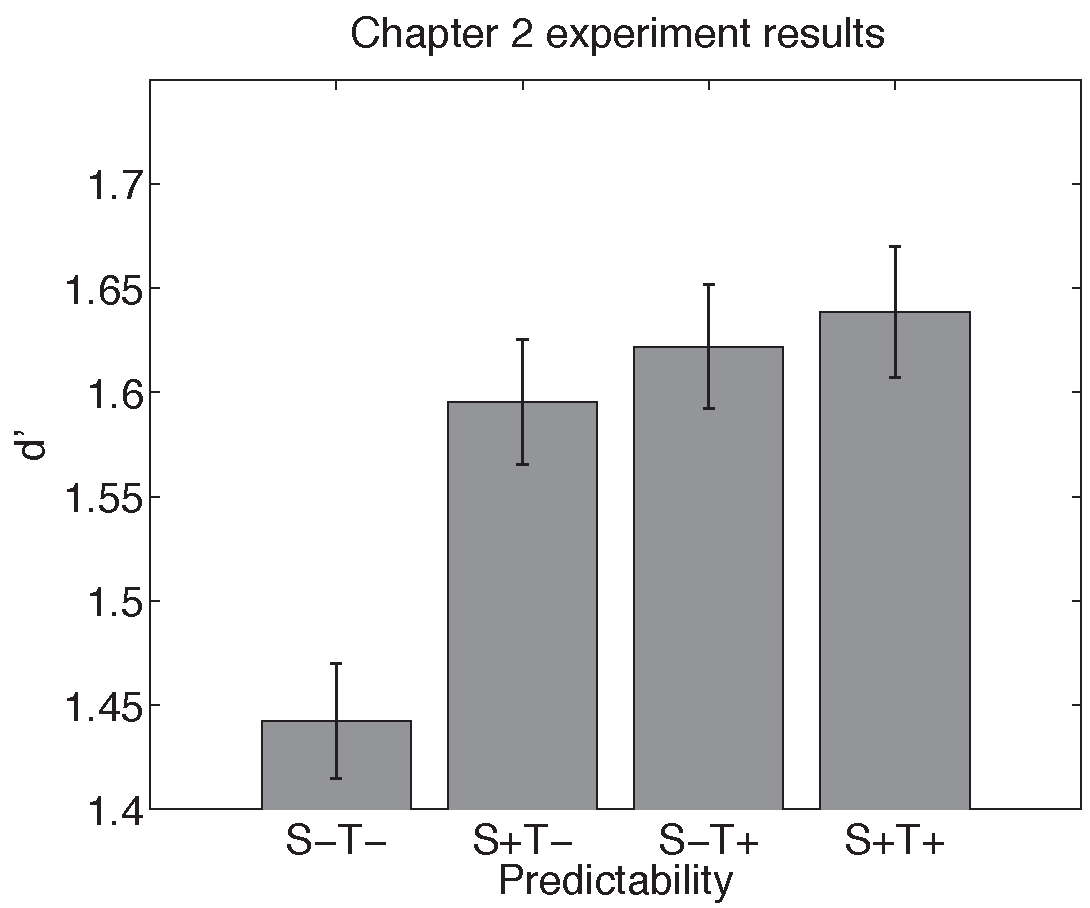
\includegraphics[width=80mm]{figs/chap_sims/pleast_dprime.pdf} &
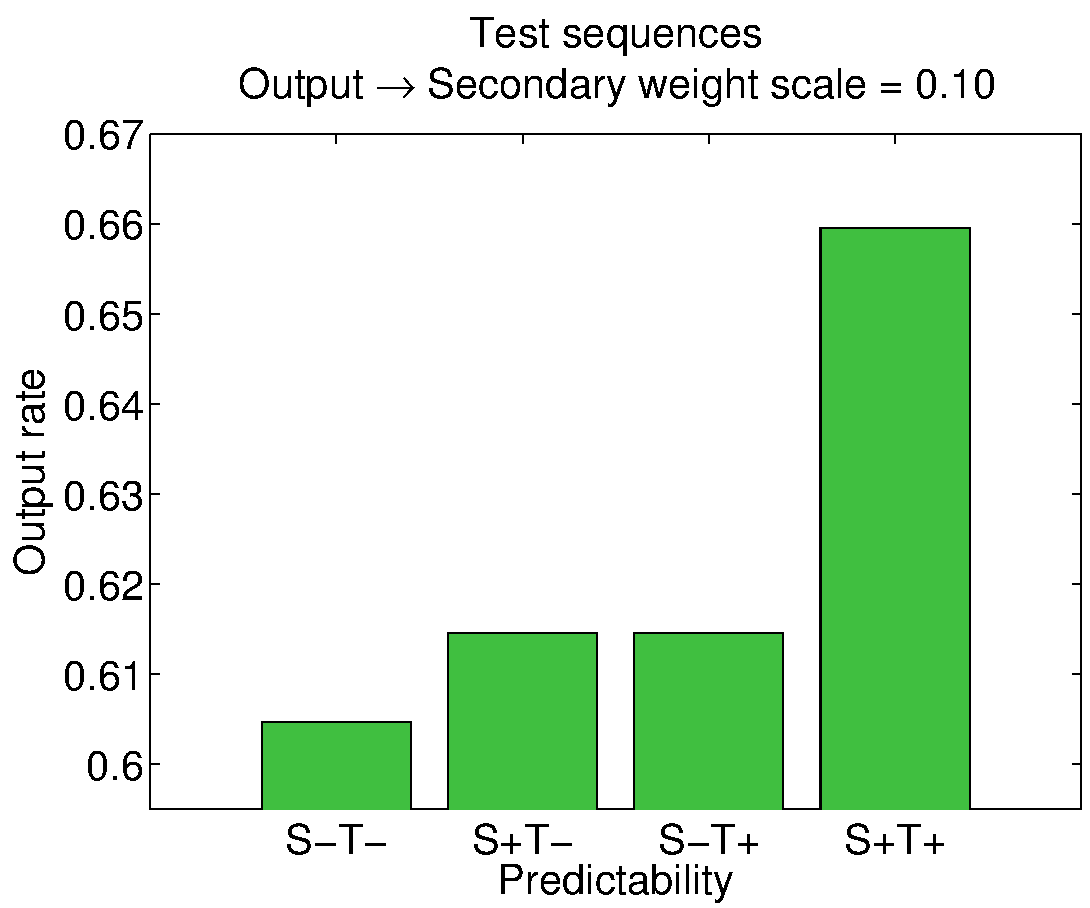
\includegraphics[width=80mm]{figs/chap_sims/sims_out_v2h_10_sterr.pdf} \\
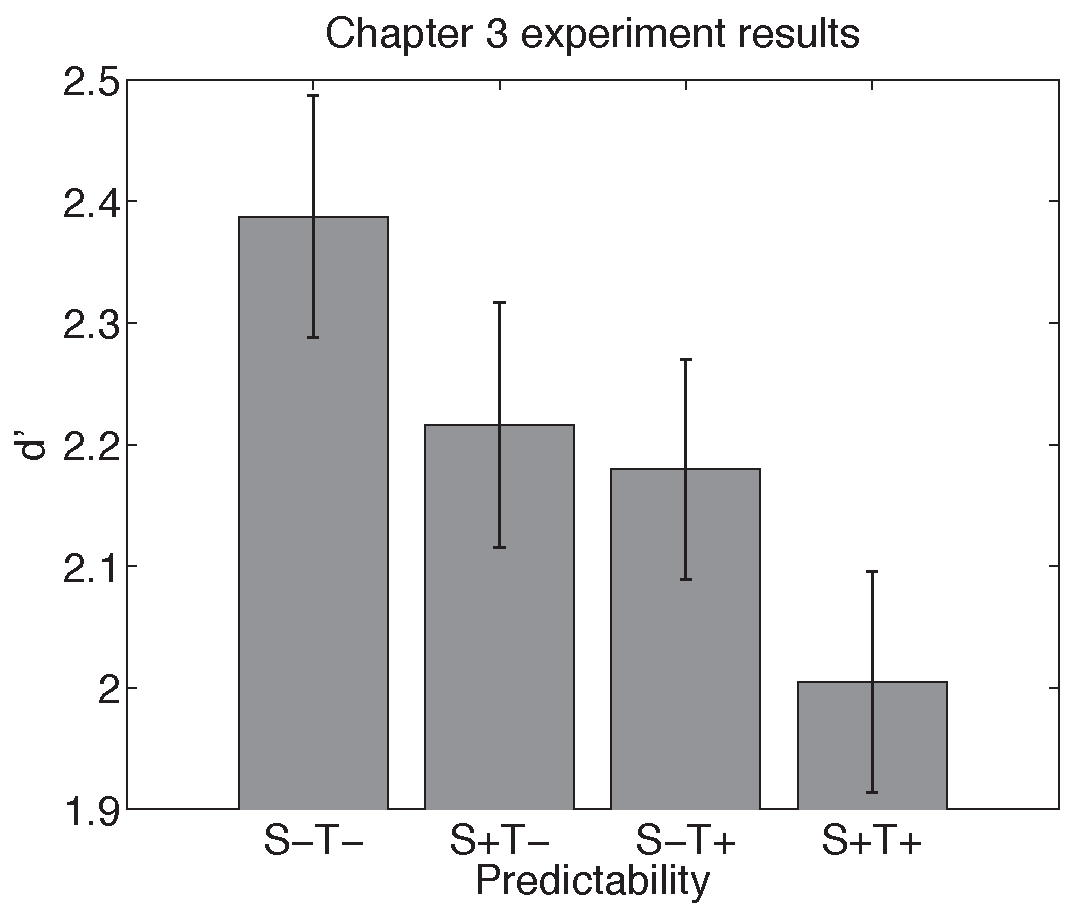
\includegraphics[width=80mm]{figs/chap_sims/bpleast_dprime.pdf} &
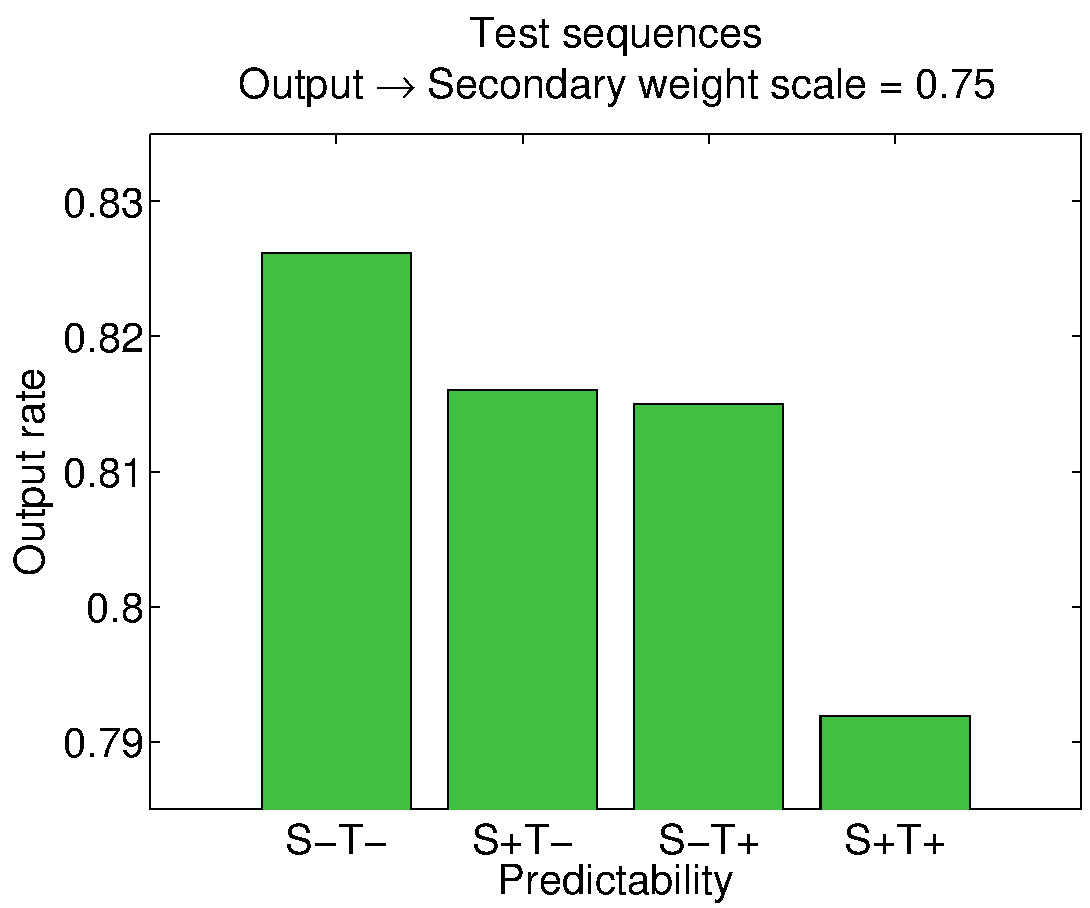
\includegraphics[width=80mm]{figs/chap_sims/sims_out_v2h_75_sterr.pdf} \\
\end{tabular}
\end{center}
\caption{Experiment and modeling results}{Chapter \ref{chap:pleast} (\textbf{top}) and \ref{chap:bpleast} (\textbf{bottom}) experiment and model results. \textit{d'} (sensitivity) was used as the common behavioral measure across experiments and the rate of the models' target output unit was used in comparison.}
\label{fig:sims_test}
\end{figure}

The Chapter \ref{chap:pleast} experiment tested subjects' ability to differentiate objects that were presented after a short series of spatiotemporally predictable or unpredictable entraining views. Subjects only ever saw 168 degrees of an object spread across 8 views on any given trial. Although feedback was given following the response on each trial, the relatively short exposure to disparate object views combined with the relatively large set of 16 possible target objects likely discouraged substantial learning. The trained model without modifications was capable of producing these results. Output unit rate was super-additive in the combined spatial and temporal predictability case as the testing sequence in this case perfectly matched the training environment in terms of spatial and temporal properties and thus maximally activated both superficial and deep units. This is a fundamental prediction of the LeabraTI model that was not present in the experimental results, but has been demonstrated in previous investigations of predictability on attentional allocation \cite{DohertyRaoMesulamEtAl05,RohenkohlGouldPessoaEtAl14}.

The Chapter \ref{chap:bpleast} experiment produced an almost complete reversal of the results from the Chapter \ref{chap:pleast} experiment. This second experiment differed from the first a number of meaningful ways. First, a smaller set of only four target objects was used. Subjects also observed each of the objects rotate completely through each of its views four times and were explicitly instructed to study the object as it rotated. No feedback was given during test trials, but each object was seen four separate times during the experiment and many subjects reported being aware of the fact that there were four unique objects. A reasonable conclusion is that these differences encouraged overtraining 
of the objects and that spatial and temporal predictability interact with this overtraining in different ways.

LeabraTI is predicated on spatiotemporal regularity and is thus somewhat inappropriate for evaluating learning under spatially and temporally unpredictable contexts. To account for the Chapter \ref{chap:bpleast} results, a simple proxy was used for overtraining the stimuli in which the scale of the weights on the Output $\rightarrow$ Secondary visual synapses was increased. Typically, a relative scale of 10\% is used on feedback projections so that feedforward inputs drive the majority of weight changes with feedback  playing a more modulatory role \cite{CrickKoch98,ShermanGuillery98}. This is crucial for the training period to prevent ``hallucinatory'' representations that can become disconnected from bottom-up inputs and produces the best testing results since model adapts its weights to the strength of inputs for each layer. 

Increasing the scale of the weights on the Output $\rightarrow$ Secondary visual synapses to 75\% produced the same reversal observed in the Chapter \ref{chap:bpleast} results in which training in the combined spatial and temporal predictability context impaired recognition relative to the completely unpredictable case. Synaptic weight scaling is one of the many effects of learning, especially when considering the long timescale self-organizing mechanisms presumed by Leabra that reinforce the most active units \cite{OReillyMunakata00,OReillyMunakataFrankEtAl12}. The full range of the reversal effect when increasing Output $\rightarrow$ Secondary visual synaptic weight scale is plotted in Figure \ref{fig:sims_ramp_distmatrix}A. Overall, the effect is graded and thus varying the amount of exposure observers have with to stimuli would probably modulate prominence of the reversal effect. 

\begin{figure}[h!]
\hspace{2mm} \textbf{A} \hspace{56mm} \textbf{B}
\begin{center}
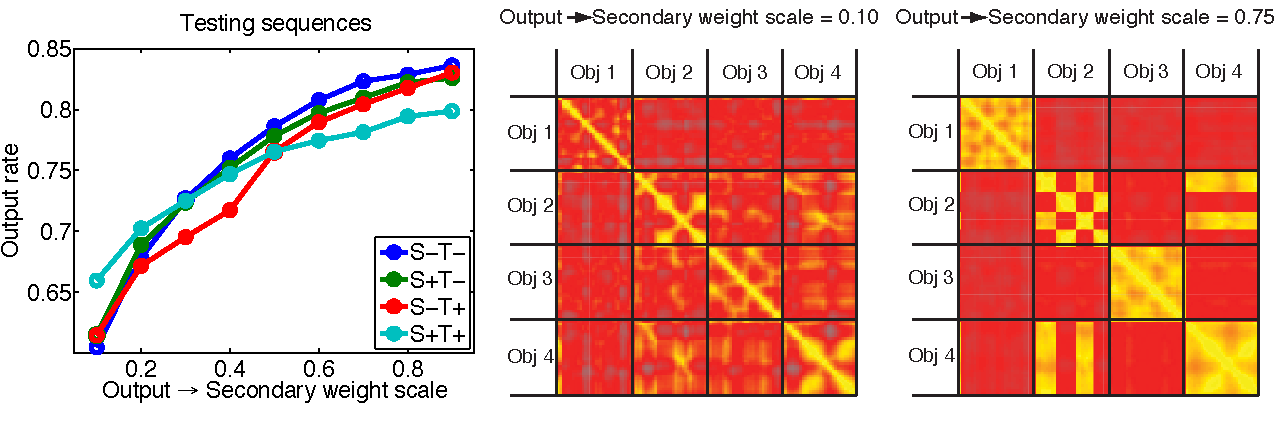
\includegraphics[width=160mm]{figs/chap_sims/sims_ramp_distmatrix_montage.pdf}
\end{center}
\caption{Effect of prolonged learning and representational similarity}{\textbf{A}: Target output rate as a function of Output $\rightarrow$ Secondary visual synaptic weight scale. Lines indicate best fit third order polynomials. \textbf{B}: Pairwise cosine over secondary visual unit minus phase activations across all views of all objects. Yellow indicates greater similarity. Results shown for both 10\% and 75\% Output $\rightarrow$ Secondary visual weight scales.}
\label{fig:sims_ramp_distmatrix}
\end{figure}

To determine the effect of learning on the representation of the objects, the cosine was used to compute a pairwise similarity metric over secondary visual unit minus phase activations across all views of all objects \abbrevcite[i.e., representational similarity,]{KriegeskorteMurRuffEtAl08}. LeabraTI training produced a representation that captures some similarity across sequential views but each view remained relatively distinct, as would be expected of V2-level representations \cite{KobatakeTanaka94,FreemanSimoncelli11}. The proxy for learning used here strengthens the synapses between secondary visual units and higher-level areas that code increasingly invariant representation. In the model, this higher-level area was a localist output layer which can be considered to be coding the same invariant representation that IT cortex does using a population code \cite{HungKreimanPoggioEtAl05,LiCoxZoccolanEtAl09}. 

The representational similarity suggests that prolonged learning causes invariance to ``trickle down'' to lower-level feature representations. This is problematic for objects that suffer from severely degenerate views such as Object 2.\footnote{In the Chapter \ref{chap:bpleast} experiment, accuracy for Object 2 suffered the most of all objects for degenerate views, falling from ceiling to below chance levels.} For Object 2, two distinct views were represented, divided by the degenerate view. However, one of these views was represented similarly to Object 4. This object confusion was less of an issue when the objects were recently acquired (10\% Output $\rightarrow$ Secondary visual weight scale) and might account for the comparatively lower performance of objects studied for prolonged periods with spatiotemporal predictability.

%\bibliographystyle{apa}
%\bibliography{ccnlab}

\end{document}